\section{Rigid Body Dynamics Lagrange Derivation}
\label{subsec2}
The multi-body model derived here aims to capture the dynamics of the tractor-sled vehicle in the current towing configuration in Fig.'s  \ref{fig:South_Pole_Traverse_Tractor_and_Sled_Configuration} and \ref{fig:Top_View_Diagram_South_Pole_Traverse}. The free body diagram for the derivation is shown in Fig. \ref{fig:Free_Body_Diagram}.
\begin{figure}[h]
    \centering
    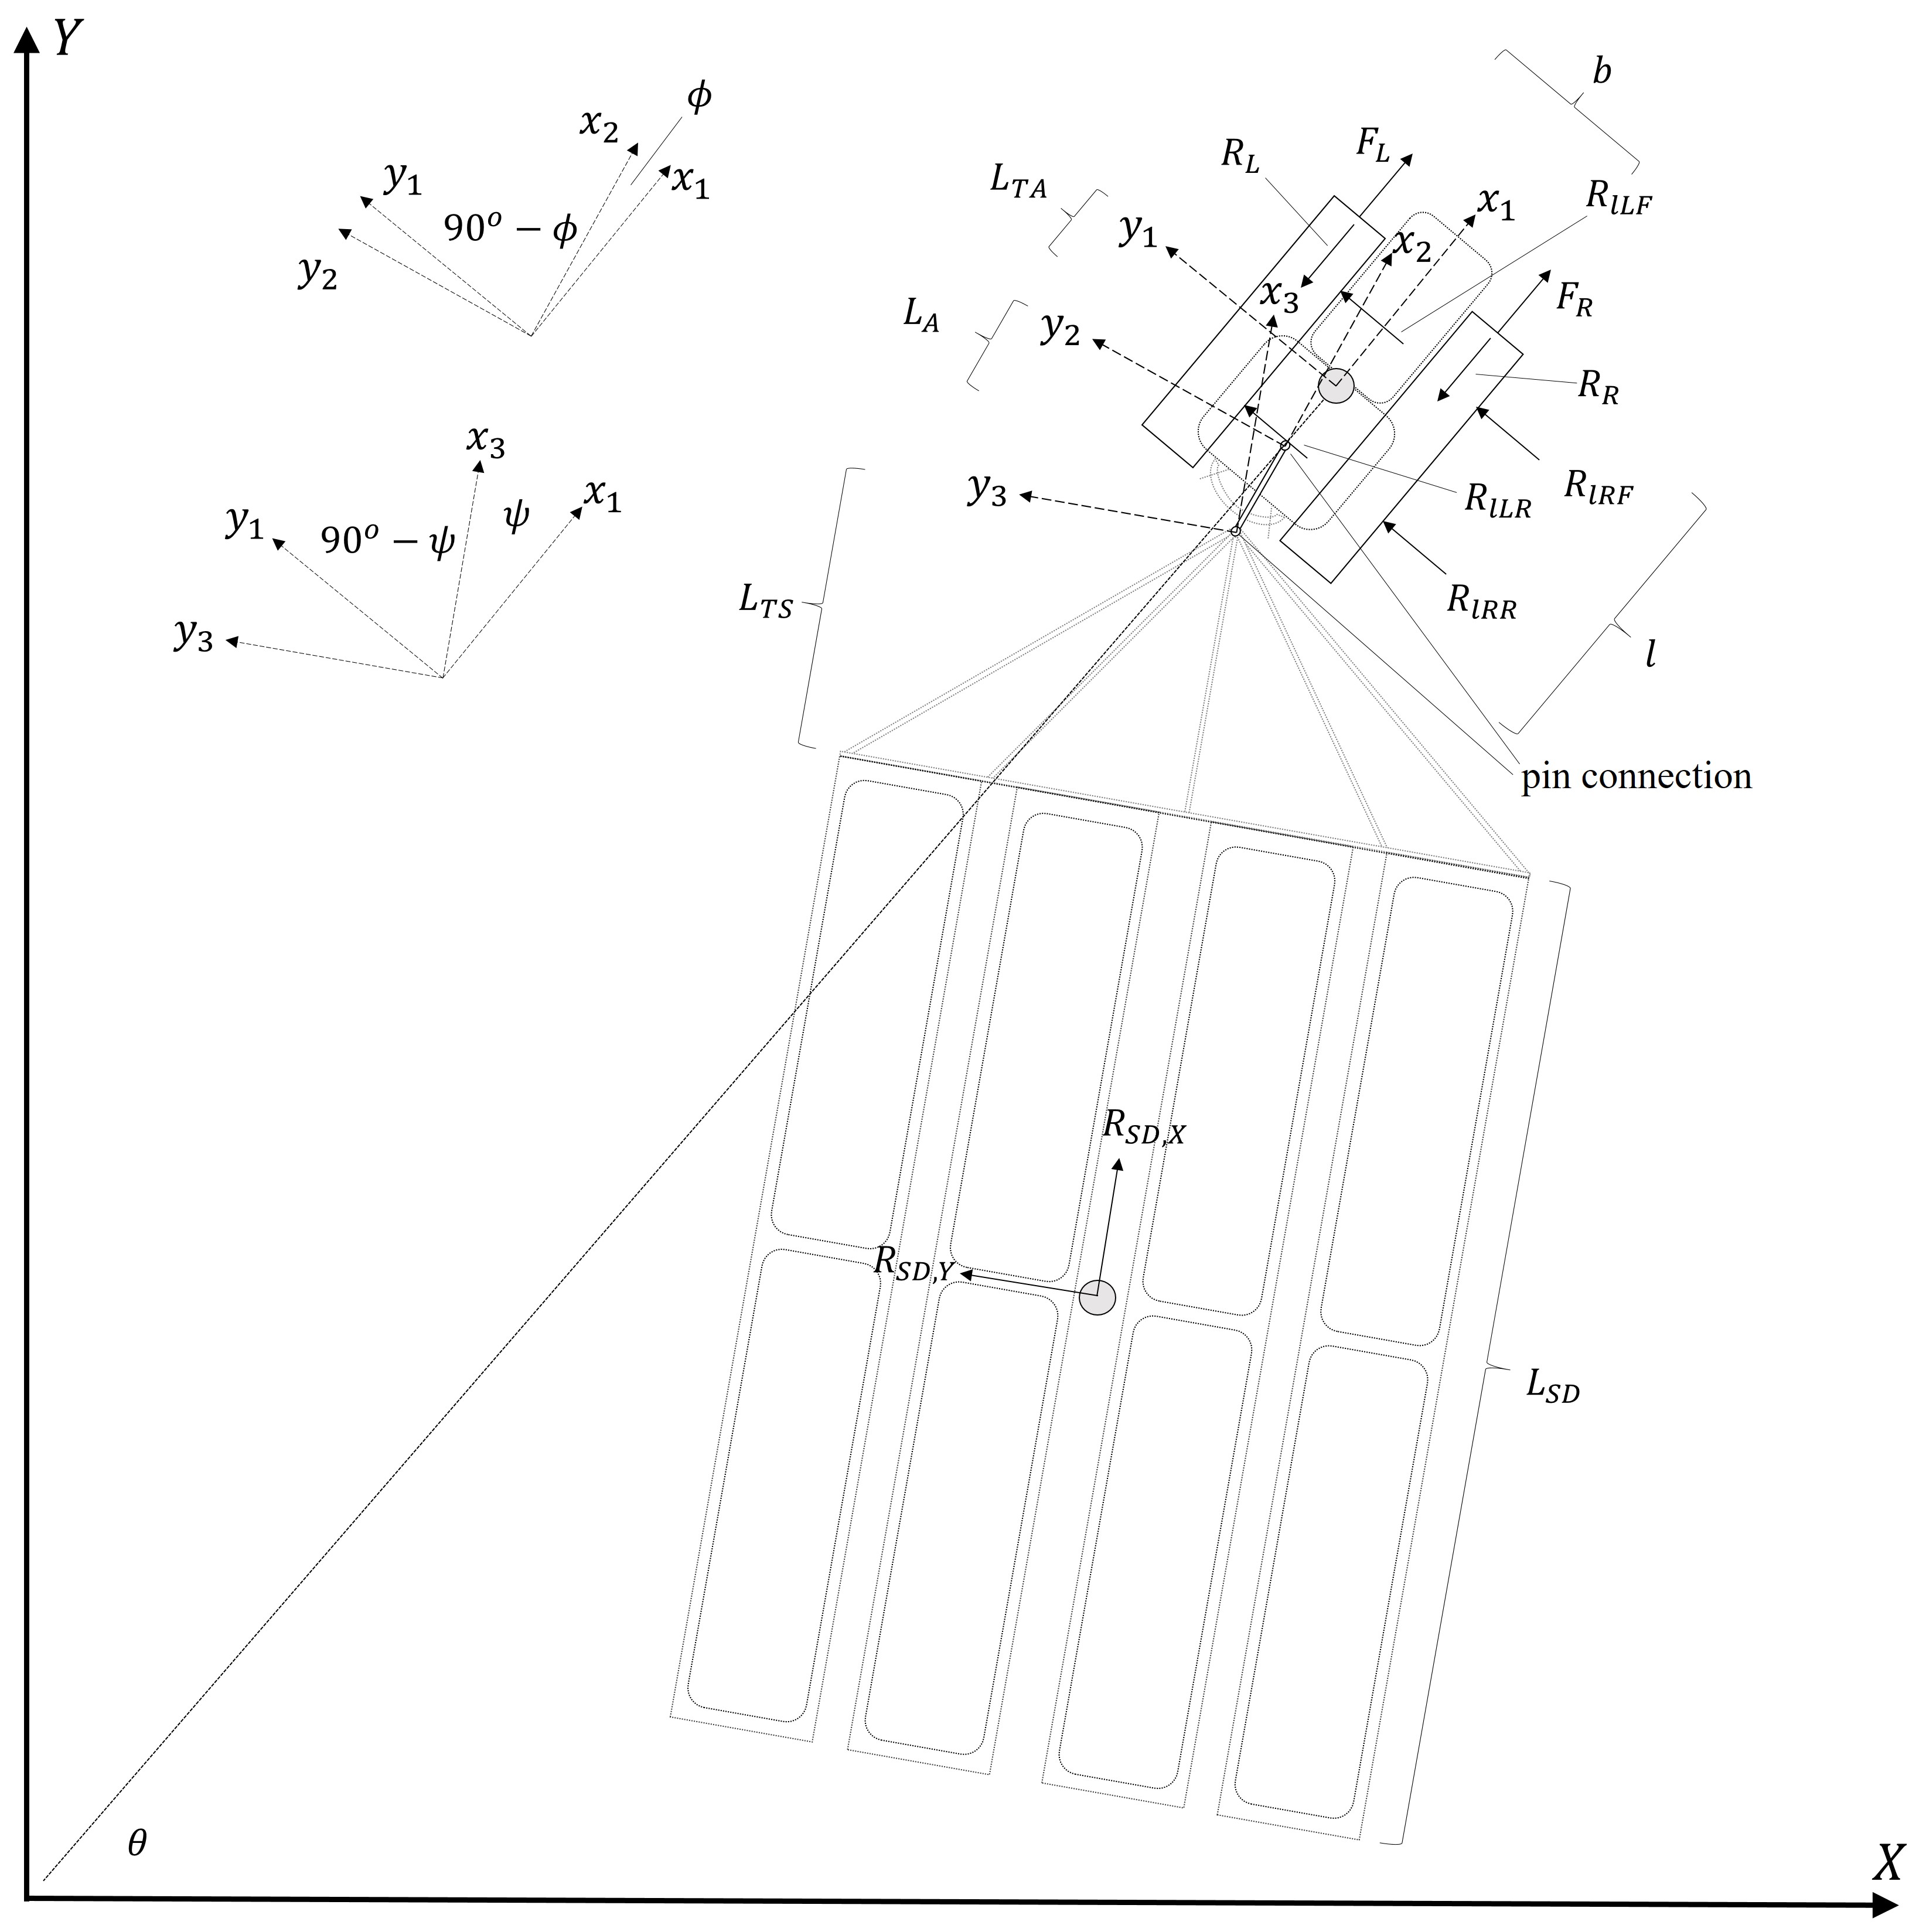
\includegraphics[width=5.5in]{Free_Body_Diagram}
    \caption{Free body diagram of the tractor-sled vehicle. Constraint forces between rigid bodies are omitted as they are not required for the Lagrangian derivation}
    \label{fig:Free_Body_Diagram}
\end{figure}
The model is derived using the Lagrangian
\begin{linenomath*}
    \begin{equation} \label{eq:lagrange}
        \frac{d}{dt}\frac{\partial T}{\partial \dot q_j} - \frac{\partial T}{\partial \dot q} = Q_j \quad \forall j
    \end{equation}
\end{linenomath*}
where $T$ is the total kinetic energy, $q_j$ is the $j^{th}$ generalized coordinate, and $Q_j$ are the generalized forces for the $j{th}$ generalized coordinate. The generalized coordinates for the system are chosen as the tractor $X$, $Y$ position in the inertial frame, the tractor heading angle $\theta$, the drawbar orientation relative to the tractor $\phi$, the sled orientation relative to the tractor $\psi$, and the left and right driver angular positions $\varphi_L$ and $\varphi_R$. The kinetic energy for any rigid body can be written as
\begin{linenomath*}
    \begin{equation}
        T = \frac{1}{2}m\mathbf{v}_G\cdot\textbf{v}_G + \frac{1}{2}\boldsymbol{\omega}_G\cdot\mathbf{H}_G
    \end{equation}
\end{linenomath*}
where $\mathbf{v}$ is the velocity, $\boldsymbol{\omega}$ is the angular velocity, $\mathbf{H}$ is angular momentum, and the subscript $G$ denotes the center of mass of the body. In this derivation, the red truss on the sled and the drawbar in grey attached to the tractor shown in Figures \ref{fig:South_Pole_Traverse_Tractor_and_Sled_Configuration}, \ref{fig:Top_View_Diagram_South_Pole_Traverse}, and \ref{fig:Free_Body_Diagram} are assumed to have negligible mass relative to the tractor ($\sim$25,000 kg) and sled load ($\sim$80,000 kg). In addition, the translational kinetic energy in the $X$, $Y$ plane and rotational kinetic energy about the $Z$ axis of the two tracks are combined with the rest of the tractor. Therefore, the kinetic energy of the system is defined as
\begin{linenomath*}
    \begin{equation}
        T = \frac{1}{2}m_T\mathbf{v}_T\cdot\textbf{v}_T + \frac{1}{2}\boldsymbol{\omega}_T\cdot\mathbf{H}_T + \frac{1}{2}m_{SD}\mathbf{v}_{SD}\cdot\textbf{v}_{SD} + \frac{1}{2}\boldsymbol{\omega}_{SD}\cdot\mathbf{H}_{SD} + \frac{1}{2}\boldsymbol{\omega}_L\cdot\mathbf{H}_L + \frac{1}{2}\boldsymbol{\omega}_R\cdot\mathbf{H}_R
    \end{equation}
\end{linenomath*}
where the subscripts $T$, $SD$, $L$, and $R$ refer to the tractor, sled, and left and rights tracks. The model being derived is planar, so the velocities of the rigid bodies and rotational kinetic energy terms are defined as
\begin{linenomath*}
    \begin{equation}
        \mathbf{v}_T = \frac{d}{dt}\mathbf{r}_{T/O} = \frac{d}{dt}(X\mathbf{I} + Y\mathbf{J})
    \end{equation}
\end{linenomath*}
\begin{linenomath*}
    \begin{multline}
        \mathbf{v}_{SD} = \frac{d}{dt}(\mathbf{r}_{SD/T} + \mathbf{r}_{T/O})
                        = \frac{d}{dt}(X\mathbf{I} + Y\mathbf{J}  - \mathbf{R}_{1/0}^TL_{TA}\mathbf{i}_1  - \mathbf{R}_{2/0}^TL_A\mathbf{i}_2) \\
                        - \mathbf{R}_{3/0}^T(\frac{1}{2}L_{SD} + L_{TS})\mathbf{i}_3
    \end{multline}
\end{linenomath*}
\begin{linenomath*}
    \begin{equation}
        \mathbf{R}_{1/0} = \begin{bmatrix} \cos\theta & \sin\theta & 0 \\ -\sin\theta & \cos\theta & 0 \\ 0 & 0 & 1 \end{bmatrix}
    \end{equation}
\end{linenomath*}
\begin{linenomath*}
    \begin{equation}
        \mathbf{R}_{2/0} = \begin{bmatrix} \cos\phi & \sin\phi & 0 \\ -\sin\phi & \cos\phi & 0 \\ 0 & 0 & 1 \end{bmatrix}\mathbf{R}_{1/0}
    \end{equation}
\end{linenomath*}
\begin{linenomath*}
    \begin{equation}
        \mathbf{R}_{3/0} = \begin{bmatrix} \cos\psi & \sin\psi & 0 \\ -\sin\psi & \cos\psi & 0 \\ 0 & 0 & 1 \end{bmatrix}\mathbf{R}_{1/0}
    \end{equation}
\end{linenomath*}
\begin{linenomath*}
    \begin{equation}
        \frac{1}{2}\boldsymbol{\omega}_G\cdot\mathbf{H}_G = \frac{1}{2}J_T\dot\theta^2
    \end{equation}
\end{linenomath*}
\begin{linenomath*}
    \begin{equation}
        \frac{1}{2}\boldsymbol{\omega}_{SD}\cdot\mathbf{H}_{SD} = \frac{1}{2}J_{SD}(\dot\theta + \dot\psi)^2
    \end{equation}
\end{linenomath*}
\begin{linenomath*}
    \begin{equation}
        \frac{1}{2}\boldsymbol{\omega}_L\cdot\mathbf{H}_L = \frac{1}{2}J_S\dot\varphi_L^2
    \end{equation}
\end{linenomath*}
\begin{linenomath*}
    \begin{equation}
        \frac{1}{2}\boldsymbol{\omega}_R\cdot\mathbf{H}_R = \frac{1}{2}J_S\dot\varphi_R^2
    \end{equation}
\end{linenomath*}
where $L_{TA}$ is the distance from the tractor CG to the drawbar, $L_A$ is the drawbar length, $L_{TS}$ is the truss length, and $L_{SD}$ is the sled length. Rotational transformation matrices are generally defined as  $\mathbf{R}_{A/B}$, where the rotation is from frame $B$ to frame $A$. From the definition of the kinetic energy, the full and partial derivatives can be taken on the left side of equation \ref{eq:lagrange} for all the generalized coordinates. The next step is to define the generalized forces, which do virtual work through virtual displacements of the generalized coordinates and are given by
\begin{linenomath*}
    \begin{equation}\label{eq:generalized_forces}
          Q_j = \sum_{P}^{} \mathbf{F}_P\cdot \frac{\partial}{\partial q_j}\mathbf{r}_{P/O}  + \sum_{K}^{} \boldsymbol{\Gamma}_K\cdot\frac{\partial}{\partial q_j}\boldsymbol{\theta}_K  \quad \forall j
    \end{equation}
\end{linenomath*}
where $\mathbf{F}_P$ is an arbitrary force vector that acts at $\mathbf{r}_{P/O}$ and $\boldsymbol{\Gamma}_K$ is an arbitrary torque vector acting on body $K$ with an angular position $\boldsymbol{\theta}_K$. For the derivation of the tractor-sled system, the terms in equation \ref{eq:generalized_forces} are evaluated as
\begin{linenomath*}
\begin{multline}
    \sum_{P}^{} \mathbf{F}_P\cdot \frac{\partial}{\partial q_j}\mathbf{r}_{P/O}
    = \mathbf{R}_{1/0}^T F_L \mathbf{i}_1 \cdot \frac{\partial}{\partial q_j}\Big(r_{T/O} + \mathbf{R}_{1/0}^T\frac{b}{2}\mathbf{j}_1\Big)
    + \mathbf{R}_{1/0}^T F_R \mathbf{i}_1 \cdot \frac{\partial}{\partial q_j}\Big(r_{T/O} - \mathbf{R}_{1/0}^T\frac{b}{2}\mathbf{j}_1\Big) \\
    - \mathbf{R}_{1/0}^T R_L \mathbf{i}_1 \cdot \frac{\partial}{\partial q_j}\Big(r_{T/O} + \mathbf{R}_{1/0}^T\Big(\frac{l}{2}\mathbf{i}_1 + \frac{b}{2}\mathbf{j}_1\Big)\Big) 
    - \mathbf{R}_{1/0}^T R_R \mathbf{i}_1 \cdot \frac{\partial}{\partial q_j}\Big(r_{T/O} + \mathbf{R}_{1/0}^T\Big(\frac{l}{2}\mathbf{i}_1 - \frac{b}{2}\mathbf{j}_1\Big)\Big) \\
    + \mathbf{R}_{1/0}^T R_{lLF} \mathbf{j}_1 \cdot \frac{\partial}{\partial q_j}\Big(r_{T/O} + \mathbf{R}_{1/0}^T\Big(\frac{l}{2}\mathbf{i}_1 + \frac{b}{2}\mathbf{j}_1\Big)\Big)
    + \mathbf{R}_{1/0}^T R_{lRF} \mathbf{j}_1 \cdot \frac{\partial}{\partial q_j}\Big(r_{T/O} + \mathbf{R}_{1/0}^T\Big(\frac{l}{2}\mathbf{i}_1 - \frac{b}{2}\mathbf{j}_1\Big)\Big) \\
    + \mathbf{R}_{1/0}^T R_{lLR} \mathbf{j}_1 \cdot \frac{\partial}{\partial q_j}\Big(r_{T/O} + \mathbf{R}_{1/0}^T\Big(-\frac{l}{2}\mathbf{i}_1 + \frac{b}{2}\mathbf{j}_1\Big)\Big)
    + \mathbf{R}_{1/0}^T R_{lRR} \mathbf{j}_1 \cdot \frac{\partial}{\partial q_j}\Big(r_{T/O} \\
    + \mathbf{R}_{1/0}^T\Big(-\frac{l}{2}\mathbf{i}_1 - \frac{b}{2}\mathbf{j}_1\Big)\Big) 
    + \mathbf{R}_{3/0}^T\Big(R_{SD,X}\mathbf{i}_3 + R_{SD,Y}\mathbf{j}_3\Big) \cdot \frac{\partial}{\partial q_j}\Big(\mathbf{r}_{SD/T} + \mathbf{r}_{T/O}\Big)
\end{multline}
\end{linenomath*}
\vspace{-25pt}
\begin{linenomath*}
    \begin{multline}
          \sum_{K}^{} \boldsymbol{\Gamma}_K\cdot\frac{\partial}{\partial q_j}\boldsymbol{\theta}_K = \Big(\tau_L - F_Lr - \zeta\dot\varphi_L\Big)\mathbf{j}_1 \cdot \frac{\partial}{\partial q_j}\Big(\varphi_L\mathbf{j}_1 + \theta\mathbf{k}_1 \Big) \\ + \Big( \tau_R - F_Rr - \zeta\dot\varphi_R \Big)\mathbf{j}_1 \cdot \frac{\partial}{\partial q_j}\Big(\varphi_R\mathbf{j}_1 + \theta\mathbf{k}_1 \Big)
    \end{multline}
\end{linenomath*}
This derivation gives the differential equations for the rigid body dynamics of the tractor sled system in terms of $\ddot X$ and $\ddot Y$. However, the motivation for the model is autonomous vehicle control, so we make substitutions to rewrite the equations in terms of $\dot v_x$ and $\dot v_y$ corresponding to the longitudinal and lateral velocity of the tractor in frame 1. The velocity of the tractor can be written as
\begin{linenomath*}
    \begin{equation}
          \dot X = v_x\cos\theta - v_y\sin\theta
    \end{equation}
\end{linenomath*}
\begin{linenomath*}
    \begin{equation}
          \dot Y = v_y\cos\theta + v_x\sin\theta
    \end{equation}
\end{linenomath*}
and then differentiated
\begin{linenomath*}
    \begin{equation}\label{eq:ddotX_sub}
          \ddot X = \dot v_x\cos\theta - \dot v_y\sin\theta - \dot\theta(v_y\cos\theta + v_x\sin\theta)
    \end{equation}
\end{linenomath*}
\begin{linenomath*}
    \begin{equation}\label{eq:ddotY_sub}
          \ddot Y = \dot v_y\cos\theta + \dot v_x\sin\theta + \dot\theta(v_x\cos\theta - v_y\sin\theta)
    \end{equation}
\end{linenomath*}
Using equations \ref{eq:ddotX_sub} and \ref{eq:ddotY_sub} for substitution, the equations of motion can be written in terms of the body fixed tractor velocities as $\mathbf{\dot x} = f(\mathbf{x})$, where the state vector is defined in equation (\ref{eq:state_vector}).
\begin{linenomath*}
    \begin{equation}\label{eq:state_vector}
        \mathbf{x} \equiv \begin{bmatrix}\begin{matrix} X & Y & \theta & \phi & \psi & v_x & v_y  & \dot\theta & \dot\phi & \dot\psi\end{matrix}\quad\begin{matrix} \dot\varphi_L & \dot\varphi_R \end{matrix}\end{bmatrix}^T
    \end{equation}
\end{linenomath*}
\begin{linenomath*}
    \begin{equation}
          \mathbf{\dot x} = \mathbf{M}^{-1}\mathbf{B}(\mathbf{x})
    \end{equation}
\end{linenomath*}
Definitions for the mass matrix $\mathbf{M}_{7x7}$ and the force vector $\mathbf{b}_{7x1}$ are given in Appendix \ref{A:MBDVMEOM}.

% --------------- Sled Force Derivation ----------------------------
In Ch. \ref{ch:RSBD} the sled loaded the drawbar of the vehicle in only one direction and its magnitude was defined as $R_{SD} = \eta m_BgN$ in eq. \ref{eq:resistanceSled}. In the multi-body model, directional sled resistances are defined in body-fixed frame 3 as $R_{SD,X}$ in the $\mathbf{i}_3$ direction and $R_{SD,Y}$ in the $\mathbf{j}_3$ direction. These forces are assumed to act in the oppposite direction of the sled's velocity and their relationship to $R_{SD}$ is given by
\begin{linenomath*}
    \begin{equation}
        R_{SD} = \sqrt{R_{SD,X}^2 + R_{SD,Y}^2}
    \end{equation}
\end{linenomath*}
Since $R_{SD,X}$ and $R_{SD,Y}$ are defined as body fixed, the velocity of the sled as defined in frame 3 must be derived. The sled velocity and resistance forces are given by
\begin{linenomath*}
    \begin{multline}
        \mathbf{v}_{SD}  = v_x\mathbf{i}_1 + v_y\mathbf{j}_1 + \mathbf{R}_{3/1}(\dot\theta\mathbf{k}_1 \times -L_{TA}\mathbf{i}_1) + \mathbf{R}_{3/2}(\dot\phi\mathbf{k}_2 \times -L_A\mathbf{i}_2) \\ + (\dot\psi\mathbf{k}_3 \times -\Big(\frac{1}{2}L_{SD} + L_{TS}\Big)\mathbf{i}_3) 
    \end{multline}
\end{linenomath*}
\begin{linenomath*}
    \begin{equation}
        \mathbf{R}_{3/1} = \begin{bmatrix} \cos\psi & \sin\psi & 0 \\ -\sin\psi & \cos\psi & 0 \\ 0 & 0 & 1 \end{bmatrix}
    \end{equation}
\end{linenomath*}
\begin{linenomath*}
    \begin{equation}
        \mathbf{R}_{3/2} = \begin{bmatrix} \cos(\psi-\phi) & \sin(\psi-\phi) & 0 \\ -\sin(\psi-\phi) & \cos(\psi-\phi) & 0 \\ 0 & 0 & 1 \end{bmatrix}
    \end{equation}
\end{linenomath*}
\begin{linenomath*}
    \begin{equation}
        R_{SD,X} = R_{SD}\Big(\frac {-\mathbf{v}_{SD} \cdot \mathbf{i}_3} { \|\mathbf{v}_{SD}\| } \Big)
    \end{equation}
\end{linenomath*}
\begin{linenomath*}
    \begin{equation}
        R_{SD,Y} = R_{SD}\Big(\frac {-\mathbf{v}_{SD} \cdot \mathbf{j}_3} { \|\mathbf{v}_{SD}\| } \Big)
    \end{equation}
\end{linenomath*}
